% !TeX document-id = {3c518733-43c3-4789-8e54-51d5112a1304}
% !TeX program = lualatex
% !BIB program = biber
% Lualatex is important to render TTF fonts; with pdflatex it's just the regular one
% ratio 16:9 -- https://tex.stackexchange.com/questions/14336/

% compile two versions, inspired by https://tex.stackexchange.com/a/1501
% use the script "compile-pdf.sh"
\newif\ifhandout
% if flags.tex does not exist, create an empty file to be able to compile in TeXstudio
\input{flags}

\ifhandout
\documentclass[12pt,aspectratio=169,handout]{beamer}
\else
\documentclass[12pt,aspectratio=169]{beamer}
\fi

% adjust for 16:9
% https://tex.stackexchange.com/questions/354022/modifying-the-margins-of-all-slides-in-beamer
\setbeamersize{text margin left=0.3cm,text margin right=4.5cm} 

%\usepackage{xcolor}

% use Metropolis as the basis theme
\usetheme[subsectionpage=progressbar]{metropolis}
% blocks with background globally
\metroset{block=fill}

% ------- Paderborn specifics ----------
\usepackage{fontspec}
%\setsansfont{karla} % looked bad, too fat
\setsansfont{Segoe UI} % looks OK-ish

% Paderborn color scheme
\definecolor{UPBUltraBlue}{RGB}{0, 37, 170}

\setbeamercolor{frametitle}{bg=white, fg=UPBUltraBlue}

% name in footer
\setbeamertemplate{frame numbering}{Prof.\ Dr.\ Ivan Habernal ~ | ~ \insertframenumber }

% adjust the background to be completely white
\setbeamercolor{background canvas}{bg=white}

% add Paderborn logo at each slide
% actually not -- it's just eating up space
%\addtobeamertemplate{frametitle}{}{%
	%\begin{tikzpicture}[remember picture,overlay]
	%	\node[anchor=north east,yshift=2pt] at (current page.north east) {
\includegraphics[height=0.9cm]{img/UPB_Logo_ENG_coloured_RGB}};
	%\end{tikzpicture}
	%}

% show TOC at every section start
\AtBeginSection{
	\frame{
		\vspace{2em}
		\sectionpage
		\hspace*{2.2em}\begin{minipage}{10cm}
			\tableofcontents[currentsection]
		\end{minipage}
		% we need the logo to show up here as well
		\begin{tikzpicture}[remember picture,overlay]
			\node[anchor=north east,yshift=2pt] at (current page.north east) {
\includegraphics[height=0.9cm]{img/UPB_Logo_ENG_coloured_RGB}};
		\end{tikzpicture}
	}
}
% ------- end of Paderborn specifics ----------


% typeset mathematics on serif
\usefonttheme[onlymath]{serif}

% better bibliography using biber as backend
\usepackage[natbib=true,backend=biber,style=authoryear-icomp,maxbibnames=30,maxcitenames=9,uniquelist=false,giveninits=true,doi=false,url=false,dashed=false,isbn=false]{biblatex}
% shared bibliography
\addbibresource{../nlpwdl-bibliography.bib}
% disable "ibid" for repeated citations
\boolfalse{citetracker}



\usepackage{xspace}


% for derivatives, https://tex.stackexchange.com/a/412442
\usepackage{physics}

\usepackage{tikz}
\usetikzlibrary{matrix, positioning}
\usetikzlibrary{angles,quotes} % for angles
\usetikzlibrary{backgrounds} % background
\usetikzlibrary{decorations.pathreplacing} % curly braces
\usetikzlibrary{calligraphy}
\usetikzlibrary{calc} % for neural nets

% for plotting functions
\usepackage{pgfplots}
\usepgfplotslibrary{dateplot}

% sub-figures
\usepackage{caption}
\usepackage{subcaption}

% book tabs
\usepackage{booktabs}


% argmin, argmax
\usepackage{amsmath}
\DeclareMathOperator*{\argmax}{arg\!\max}
\DeclareMathOperator*{\argmin}{arg\!\min}
% softmax
\DeclareMathOperator*{\softmax}{soft\!\max}

% bold math
\usepackage{bm}

% for \mathclap
\usepackage{mathtools}

% algorithms
\usepackage[noend]{algpseudocode}


% for neurons and layers in tikz
\tikzset{
	neuron/.style={draw, rectangle, inner sep=2pt, minimum width=0.75cm, fill=blue!20},
	param/.style={draw, rectangle, inner sep=2pt, minimum width=0.75cm, fill=green!20},
	constant/.style={draw, rectangle, inner sep=2pt, minimum width=0.75cm, fill=black!15},
	% for citation nodes right top
	ref/.style={anchor = north east, text width=7.8cm, yshift=-1.3cm, xshift=-0.2cm, scale=0.5},
	state/.style={rectangle, inner sep=2pt, minimum width=0.75cm, fill=black!5},
}

% for strike-through text (added in Lecture 06)
\usepackage[normalem]{ulem}

% added in Lecture 7
% RNN
\DeclareMathOperator*{\rnn}{RNN}
% RNN star
\DeclareMathOperator*{\rnnstar}{RNN^{*}}
% bi-RNN
\DeclareMathOperator*{\birnn}{biRNN}

\title{Natural Language Processing with Deep Learning}
\subtitle{Lecture 7 --- Text classification 4: Recurrent neural networks}
\date{November 24, 2023}
\author{Prof.\ Dr.\ Ivan Habernal}
\institute{Natural Language Processing Group 
	\hfill 
\includegraphics[height=1.4cm]{img/UPB_Logo_ENG_coloured_RGB} \\
	Paderborn University \\
	We focus on Trustworthy Human Language Technologies \hfill \texttt{www.trusthlt.org} }



\begin{document}
	
	\maketitle
	
	\begin{frame}{Motivation}
		
		Language data -- working with sequences (of tokens, characters, etc.)
		
		MLP -- fixed input vector size
		
		\bigskip
		
		\pause
		
		How we dealt with it
		
		\begin{itemize}
			\item Vector concatenation
			\item Vector addition/averaging (CBOW)
			\item Limiting context (e.g., Markov property)
		\end{itemize}
		
		What we want to really work with: Sequence of inputs, fixed-size output(s)
		
	\end{frame}
	
	
	\section{Recurrent Neural Networks (RNN) abstraction}
	
	\begin{frame}{RNN abstraction}
		
		We have a sequence of $n$ \textbf{input} vectors $\bm{x_{1:n}} = \bm{x_1}, \ldots, \bm{x_n}$
		
		Each input vector has the same dimension $d_{in}: \bm{x_i} \in \mathbb{R}^{d_{in}}$
		
		\bigskip
		
		What might $\bm{x_i}$ contain?
		\begin{itemize}
			\item Typically a word embedding of token $i$, but could be any arbitrary input, e.g., one-hot encoding of token $i$
		\end{itemize}
		\bigskip
		
		\pause
		
		We have a single \textbf{output} $d_{out}$-dimensional vector $\bm{y_n} \in \mathbb{R}^{d_{out}}$
		
		\bigskip
		
		RNN is a function from input to output
		$$
		\bm{y_n} = \rnn (\bm{x_{1:n}})
		$$
	\end{frame}
	
	
	\begin{frame}{RNN in fact returns a sequence of outputs}
		
		RNN definition: $\bm{y_n} = \rnn (\bm{x_{1:n}})$
		
		Let's have $n = 3$, so our input sequence is $\bm{x_{1}}, \bm{x_2}, \bm{x_3}$:
		$$
		\bm{y_2} = \rnn (\bm{x_{1}}, \bm{x_2}, \bm{x_3})
		$$
		
		\pause
		
		But our input sequence also contains $\bm{x_{1}}, \bm{x_2}$, so:
		$$
		\bm{y_2} = \rnn (\bm{x_{1}}, \bm{x_2})
		$$
		
		Which makes $\rnn$ outputting a vector $\bm{y_i} \in \mathbb{R}^{d_{out}}$ at each position $i \in (1, \ldots, n)$
		
		Let's call this sequence-outputting function $\rnnstar$:
		$$
		\bm{y_{1:n}} = \rnnstar (\bm{x_{1:n}})
		$$
		
	\end{frame}
	
	
	
	\begin{frame}{Recap}
		
		For a sequence of input vectors  $\bm{x_{1:i}}$
		$$
		\bm{y_i} = \rnn (\bm{x_{1:i}}) \qquad
		\bm{y_{1:n}} = \rnnstar (\bm{x_{1:n}})
		$$
		
		\pause
		
		Without knowing what $\rnn$ actually is, what are the advantages?
		\pause
		\begin{itemize}
			\item Each output $\bm{y_i}$ takes into account the entire history $\bm{x_{1:i}}$ without Markov property
		\end{itemize}
		
		What to do with $\bm{y_n}$ or $\bm{y_{1:n}}$?
		\pause
		\begin{itemize}
			\item Use for further prediction, e.g., plug into $\softmax$, MLP, etc.
		\end{itemize}
		
	\end{frame}
	
	
	\begin{frame}{Underlying mechanism of RNNs --- states}
		For ``passing information'' from one position to the next, i.e.\ from
		$$\bm{y_i} = \rnn (\bm{x_{1:i}})$$
		to
		$$\bm{y_{i+1}} = \rnn (\bm{x_{1:i+1}})$$
		we use a ``state'' vector
		$$\bm{s_i} \in \mathbb{R}^{d_{state}}$$
	\end{frame}
	
	
	
	\begin{frame}{Define RNN recursively --- Computing current state}
		At each step $i \in (1, \ldots, n)$ we have
		\begin{itemize}
			\item Current input vector $\bm{x_i}$
			\item Vector of the previous state $\bm{s_{i - 1}}$\footnote{Initial state vector $\bm{s_0}$ --- often omitted, assumed to be zero-filled}
		\end{itemize}
		and compute
		\begin{itemize}
			\item Current state $\bm{s_i}$
		\end{itemize}
		$$
		\bm{s_i} = R(\bm{s_{i-1}}, \bm{x_i}) \qquad \text{(we will specify $R$ later)}
		$$
		
	\end{frame}
	
	
	\begin{frame}{Define RNN recursively --- Computing current output}
		At each step $i \in (1, \ldots, n)$ we have
		\begin{itemize}
			\item Current input vector $\bm{x_i}$
			\item Vector of the previous state $\bm{s_{i - 1}}$
		\end{itemize}
		and compute
		\begin{itemize}
			\item Current state $\bm{s_i} = R(\bm{s_{i-1}}, \bm{x_i})$
			\item Current output $\bm{y_i}$
		\end{itemize}
		$$
		\bm{y_i} = O(\bm{s_i}) \qquad \text{(we will specify $O$ later)}
		$$
		
	\end{frame}
	
	
	\begin{frame}{Summary}
		At each step $i \in (1, \ldots, n)$ we have
		\begin{itemize}
			\item Current input $\bm{x_i}$ and previous state $\bm{s_{i - 1}}$
		\end{itemize}
		and compute
		\begin{itemize}
			\item $\bm{s_i} = R(\bm{s_{i-1}}, \bm{x_i})$ and $\bm{y_i}  = O(\bm{s_i})$
		\end{itemize}
		
		The functions $R$ and $O$ are the same for each position $i$
		
		\begin{block}{RNN}
			$\bm{y_{1:n}} = \rnnstar (\bm{x_{1:n}}, \bm{s_0})
			\qquad
			\bm{s_i} = R(\bm{s_{i-1}}, \bm{x_i})
			\qquad
			\bm{y_i}  = O(\bm{s_i})$
		\end{block}
		
		
	\end{frame}
	
	
	\begin{frame}{Graphical visualization of abstract RNN (recursive)}
		
		\begin{figure}
			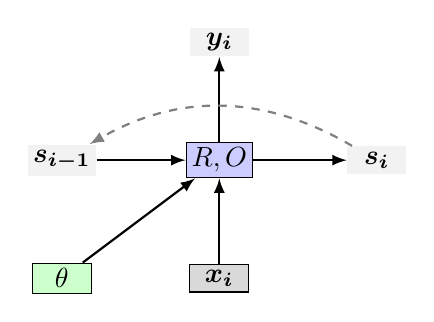
\begin{tikzpicture}	
				%\node (a1) [draw, circle, inner sep=0pt, minimum width=0.75cm, fill=green!20] {$a_1$};
				
				\node (s0) [state]{$\bm{s_{i-1}}$};
				\node (e) [param, below of=s0, yshift=-0.5cm] {$\theta$};
				
				\node (ro) [neuron, right of=s0, xshift=1cm] {$R, O$};
				\node (si) [state, right of=ro, xshift=1cm] {$\bm{s_{i}}$};
				\node (xi) [constant, below of=ro, yshift=-0.5cm] {$\bm{x_{i}}$};
				\node(yi) [state, above of=ro, yshift=0.5cm] {$\bm{y_i}$};
				
				\begin{scope}[thick, black, ->, >=latex]
					\draw (s0) -- (ro);
					\draw(xi) -- (ro);
					\draw(e) -- (ro);
					\draw(ro) -- (si);
					\draw(ro) -- (yi);
				\end{scope}
				\draw [thick, dashed, gray, ->, >=latex] (si) to [bend right] (s0);
				
			\end{tikzpicture}
		\end{figure}
		
	\end{frame}
	
	
	\begin{frame}{Graphical visualization of abstract RNN (unrolled)}
		
		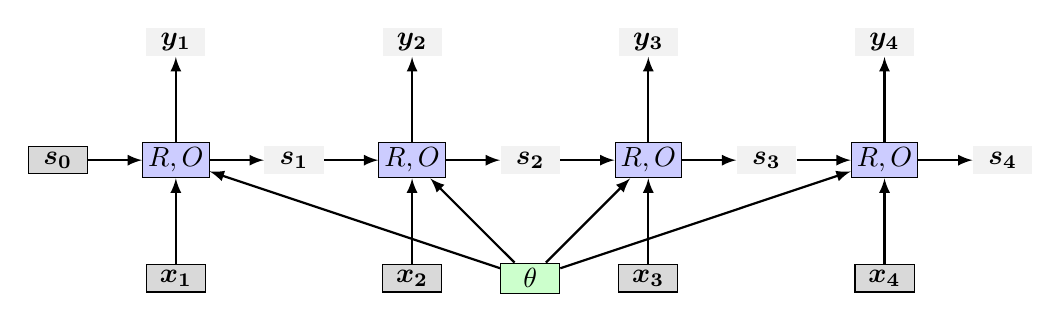
\begin{tikzpicture}	
			%\node (a1) [draw, circle, inner sep=0pt, minimum width=0.75cm, fill=green!20] {$a_1$};
			
			\node (s0) [constant]{$\bm{s_0}$};
			
			\node (ro1) [neuron, right of=s0, xshift=0.5cm] {$R, O$};
			\node (s1) [state, right of=ro1, xshift=0.5cm] {$\bm{s_1}$};
			\node (x1) [constant, below of=ro1, yshift=-0.5cm] {$\bm{x_1}$};
			\node(y1) [state, above of=ro1, yshift=0.5cm] {$\bm{y_1}$};
			
			\node (ro2) [neuron, right of=s1, xshift=0.5cm] {$R, O$};
			\node (s2) [state, right of=ro2, xshift=0.5cm] {$\bm{s_2}$};
			\node (x2) [constant, below of=ro2, yshift=-0.5cm] {$\bm{x_2}$};
			\node(y2) [state, above of=ro2, yshift=0.5cm] {$\bm{y_2}$};
			
			\node (ro3) [neuron, right of=s2, xshift=0.5cm] {$R, O$};
			\node (s3) [state, right of=ro3, xshift=0.5cm] {$\bm{s_3}$};
			\node (x3) [constant, below of=ro3, yshift=-0.5cm] {$\bm{x_3}$};
			\node(y3) [state, above of=ro3, yshift=0.5cm] {$\bm{y_3}$};
			
			\node (ro4) [neuron, right of=s3, xshift=0.5cm] {$R, O$};
			\node (s4) [state, right of=ro4, xshift=0.5cm] {$\bm{s_4}$};
			\node (x4) [constant, below of=ro4, yshift=-0.5cm] {$\bm{x_4}$};
			\node(y4) [state, above of=ro4, yshift=0.5cm] {$\bm{y_4}$};
			
			\node (e) [param, below of=s2, yshift=-0.5cm] {$\theta$};
			
			
			\begin{scope}[thick, black, ->, >=latex]
				\draw (s0) -- (ro1);
				\draw(x1) -- (ro1);
				\draw(e) -- (ro1);
				\draw(ro1) -- (s1);
				\draw(ro1) -- (y1);
				
				\draw (s1) -- (ro2);
				\draw(x2) -- (ro2);
				\draw(e) -- (ro2);
				\draw(ro2) -- (s2);
				\draw(ro2) -- (y2);
				
				\draw (s2) -- (ro3);
				\draw(x3) -- (ro3);
				\draw(e) -- (ro3);
				\draw(ro3) -- (s3);
				\draw(ro3) -- (y3);
				
				\draw (s3) -- (ro4);
				\draw(x4) -- (ro4);
				\draw(e) -- (ro4);
				\draw(ro4) -- (s4);
				\draw(ro4) -- (y4);
				
			\end{scope}
			
		\end{tikzpicture}
		
		\bigskip
		\pause
		Note that $\theta$ (parameters) are ``shared" (the same) for all positions
		
		
	\end{frame}
	
	
	\subsection{RNN as `acceptor' or `encoder'}
	
	
	\begin{frame}{Supervision on the last output}
		
		
		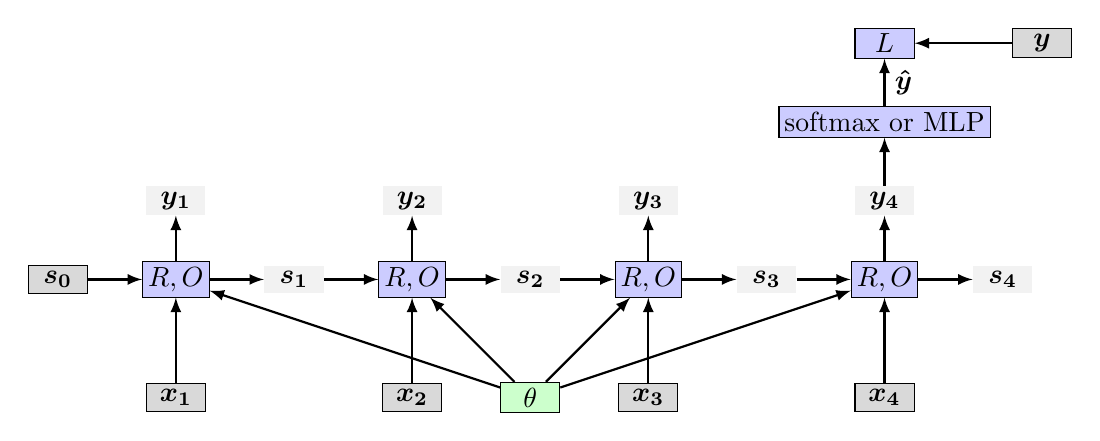
\begin{tikzpicture}	
			%\node (a1) [draw, circle, inner sep=0pt, minimum width=0.75cm, fill=green!20] {$a_1$};
			
			\node (s0) [constant]{$\bm{s_0}$};
			
			\node (ro1) [neuron, right of=s0, xshift=0.5cm] {$R, O$};
			\node (s1) [state, right of=ro1, xshift=0.5cm] {$\bm{s_1}$};
			\node (x1) [constant, below of=ro1, yshift=-0.5cm] {$\bm{x_1}$};
			\node(y1) [state, above of=ro1, yshift=0cm] {$\bm{y_1}$};
			
			\node (ro2) [neuron, right of=s1, xshift=0.5cm] {$R, O$};
			\node (s2) [state, right of=ro2, xshift=0.5cm] {$\bm{s_2}$};
			\node (x2) [constant, below of=ro2, yshift=-0.5cm] {$\bm{x_2}$};
			\node(y2) [state, above of=ro2, yshift=0cm] {$\bm{y_2}$};
			
			\node (ro3) [neuron, right of=s2, xshift=0.5cm] {$R, O$};
			\node (s3) [state, right of=ro3, xshift=0.5cm] {$\bm{s_3}$};
			\node (x3) [constant, below of=ro3, yshift=-0.5cm] {$\bm{x_3}$};
			\node(y3) [state, above of=ro3, yshift=0cm] {$\bm{y_3}$};
			
			\node (ro4) [neuron, right of=s3, xshift=0.5cm] {$R, O$};
			\node (s4) [state, right of=ro4, xshift=0.5cm] {$\bm{s_4}$};
			\node (x4) [constant, below of=ro4, yshift=-0.5cm] {$\bm{x_4}$};
			\node(y4) [state, above of=ro4, yshift=0cm] {$\bm{y_4}$};
			
			\node (e) [param, below of=s2, yshift=-0.5cm] {$\theta$};
			
			
			\node (mlp) [neuron, above of=y4] {$\softmax$ or MLP};
			
			\node (l) [neuron, above of=mlp] {$L$};
			\node (y) [constant, right of=l, xshift=1cm] {$\bm{y}$};
			
			
			\begin{scope}[thick, black, ->, >=latex]
				\draw (s0) -- (ro1);
				\draw(x1) -- (ro1);
				\draw(e) -- (ro1);
				\draw(ro1) -- (s1);
				\draw(ro1) -- (y1);
				
				\draw (s1) -- (ro2);
				\draw(x2) -- (ro2);
				\draw(e) -- (ro2);
				\draw(ro2) -- (s2);
				\draw(ro2) -- (y2);
				
				\draw (s2) -- (ro3);
				\draw(x3) -- (ro3);
				\draw(e) -- (ro3);
				\draw(ro3) -- (s3);
				\draw(ro3) -- (y3);
				
				\draw (s3) -- (ro4);
				\draw(x4) -- (ro4);
				\draw(e) -- (ro4);
				\draw(ro4) -- (s4);
				\draw(ro4) -- (y4);
				
				\draw (y4) -- (mlp);
				\draw (mlp) -- (l) node [midway, right] {$\bm{\hat{y}}$};
				\draw (y) -- (l);
				
			\end{scope}
			
			
			
		\end{tikzpicture}
		
		
		
		The loss is computed on the final output (e.g., directly on $\bm{y_n}$ or by putting $\bm{y_n}$ through MLP)
		
		
		
	\end{frame}
	
	
	\subsection{RNN as `transducer'}
	
	
	\begin{frame}{Supervision on each output}
		
		
		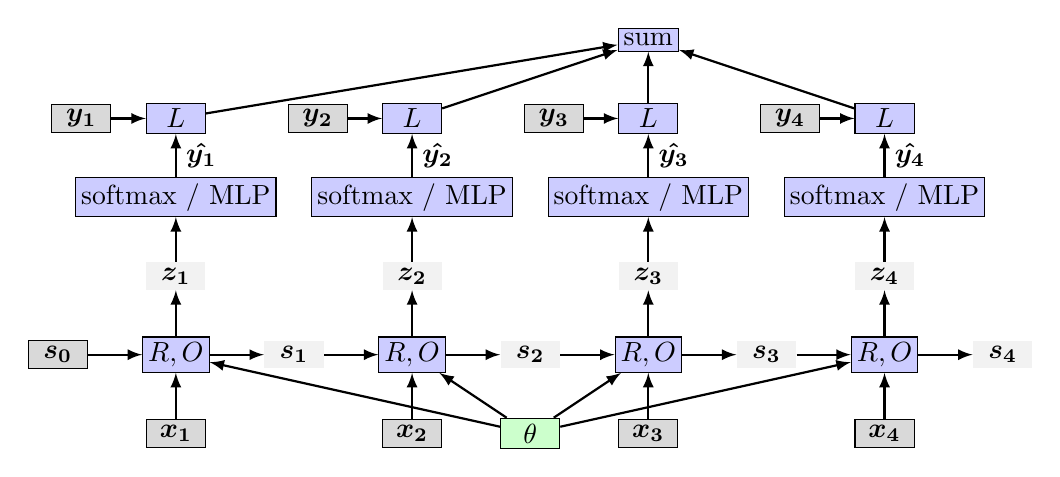
\begin{tikzpicture}	
			%\node (a1) [draw, circle, inner sep=0pt, minimum width=0.75cm, fill=green!20] {$a_1$};
			
			\node (s0) [constant]{$\bm{s_0}$};
			
			\node (ro1) [neuron, right of=s0, xshift=0.5cm] {$R, O$};
			\node (s1) [state, right of=ro1, xshift=0.5cm] {$\bm{s_1}$};
			\node (x1) [constant, below of=ro1, yshift=-0cm] {$\bm{x_1}$};
			\node(y1) [state, above of=ro1, yshift=0cm] {$\bm{z_1}$};
			
			\node (ro2) [neuron, right of=s1, xshift=0.5cm] {$R, O$};
			\node (s2) [state, right of=ro2, xshift=0.5cm] {$\bm{s_2}$};
			\node (x2) [constant, below of=ro2, yshift=-0cm] {$\bm{x_2}$};
			\node(y2) [state, above of=ro2, yshift=0cm] {$\bm{z_2}$};
			
			\node (ro3) [neuron, right of=s2, xshift=0.5cm] {$R, O$};
			\node (s3) [state, right of=ro3, xshift=0.5cm] {$\bm{s_3}$};
			\node (x3) [constant, below of=ro3, yshift=-0cm] {$\bm{x_3}$};
			\node(y3) [state, above of=ro3, yshift=0cm] {$\bm{z_3}$};
			
			\node (ro4) [neuron, right of=s3, xshift=0.5cm] {$R, O$};
			\node (s4) [state, right of=ro4, xshift=0.5cm] {$\bm{s_4}$};
			\node (x4) [constant, below of=ro4, yshift=-0cm] {$\bm{x_4}$};
			\node(y4) [state, above of=ro4, yshift=0cm] {$\bm{z_4}$};
			
			\node (e) [param, below of=s2, yshift=-0cm] {$\theta$};
			
			
			\node (mlp1) [neuron, above of=y1] {$\softmax$ / MLP};
			\node (mlp2) [neuron, above of=y2] {$\softmax$ / MLP};
			\node (mlp3) [neuron, above of=y3] {$\softmax$ / MLP};
			\node (mlp4) [neuron, above of=y4] {$\softmax$ / MLP};
			
			\node (l1) [neuron, above of=mlp1] {$L$};
			\node (l2) [neuron, above of=mlp2] {$L$};
			\node (l3) [neuron, above of=mlp3] {$L$};
			\node (l4) [neuron, above of=mlp4] {$L$};
			
			\node (yg1) [constant, left of=l1, xshift=-0.2cm] {$\bm{y_1}$};
			\node (yg2) [constant, left of=l2, xshift=-0.2cm] {$\bm{y_2}$};
			\node (yg3) [constant, left of=l3, xshift=-0.2cm] {$\bm{y_3}$};
			\node (yg4) [constant, left of=l4, xshift=-0.2cm] {$\bm{y_4}$};
			
			\node (sum) [neuron, above of=l3] {sum};
			
			\begin{scope}[thick, black, ->, >=latex]
				\draw (s0) -- (ro1);
				\draw(x1) -- (ro1);
				\draw(e) -- (ro1);
				\draw(ro1) -- (s1);
				\draw(ro1) -- (y1);
				
				\draw (s1) -- (ro2);
				\draw(x2) -- (ro2);
				\draw(e) -- (ro2);
				\draw(ro2) -- (s2);
				\draw(ro2) -- (y2);
				
				\draw (s2) -- (ro3);
				\draw(x3) -- (ro3);
				\draw(e) -- (ro3);
				\draw(ro3) -- (s3);
				\draw(ro3) -- (y3);
				
				\draw (s3) -- (ro4);
				\draw(x4) -- (ro4);
				\draw(e) -- (ro4);
				\draw(ro4) -- (s4);
				\draw(ro4) -- (y4);
				
				\draw (y1) -- (mlp1);
				\draw (y2) -- (mlp2);
				\draw (y3) -- (mlp3);
				\draw (y4) -- (mlp4);
				
				\draw (mlp1) -- (l1) node [midway, right] {$\bm{\hat{y_1}}$};
				\draw (mlp2) -- (l2) node [midway, right] {$\bm{\hat{y_2}}$};
				\draw (mlp3) -- (l3) node [midway, right] {$\bm{\hat{y_3}}$};
				\draw (mlp4) -- (l4) node [midway, right] {$\bm{\hat{y_4}}$};
				
				\draw (yg1) -- (l1);
				\draw (yg2) -- (l2);
				\draw (yg3) -- (l3);
				\draw (yg4) -- (l4);
				
				\draw (l1) -- (sum);
				\draw (l2) -- (sum);
				\draw (l3) -- (sum);
				\draw (l4) -- (sum);
				
			\end{scope}
			
			
			
		\end{tikzpicture}
		
		For sequence tagging --- loss on each position, overall network's loss simply as a sum of losses
		
		
	\end{frame}
	
	\begin{frame}{Bi-directional RNNs}
		Simple idea: Run one RNN from left-to-right (forward, $f$) and another RNN from right-to-left (backward, $b$), and concatenate
		$$
		\birnn (\bm{x_{1:i}}, i) = \bm{y_i} = [
		\rnn_f(\bm{x_{1:i}});
		\rnn_b(\bm{x_{n:i}})
		]
		$$
		
		Both for encoder (concatenate the last outputs) and transducer (concatenate each step's output)
		
	\end{frame}
	
	\begin{frame}{But what is happening `inside' $R$ and $O$?}
		\begin{figure}
			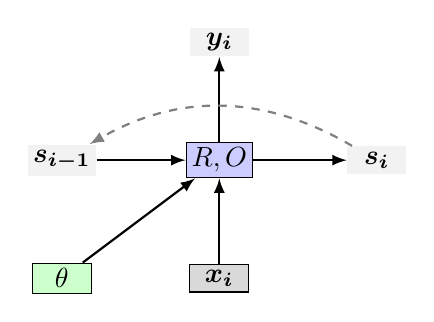
\begin{tikzpicture}	
				%\node (a1) [draw, circle, inner sep=0pt, minimum width=0.75cm, fill=green!20] {$a_1$};
				
				\node (s0) [state]{$\bm{s_{i-1}}$};
				\node (e) [param, below of=s0, yshift=-0.5cm] {$\theta$};
				
				\node (ro) [neuron, right of=s0, xshift=1cm] {$R, O$};
				\node (si) [state, right of=ro, xshift=1cm] {$\bm{s_{i}}$};
				\node (xi) [constant, below of=ro, yshift=-0.5cm] {$\bm{x_{i}}$};
				\node(yi) [state, above of=ro, yshift=0.5cm] {$\bm{y_i}$};
				
				\begin{scope}[thick, black, ->, >=latex]
					\draw (s0) -- (ro);
					\draw(xi) -- (ro);
					\draw(e) -- (ro);
					\draw(ro) -- (si);
					\draw(ro) -- (yi);
				\end{scope}
				\draw [thick, dashed, gray, ->, >=latex] (si) to [bend right] (s0);
				
			\end{tikzpicture}
		\end{figure}
	\end{frame}
	
	\section{RNN architectures}
	
	
	\subsection{Simple RNN}
	
	\begin{frame}{Elman Network or Simple-RNN (S-RNN)}
		\begin{figure}
			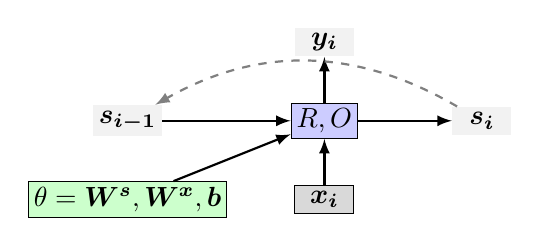
\begin{tikzpicture}	
				%\node (a1) [draw, circle, inner sep=0pt, minimum width=0.75cm, fill=green!20] {$a_1$};
				
				\node (s0) [state]{$\bm{s_{i-1}}$};
				\node (e) [param, below of=s0] {$\theta = \bm{W^s}, \bm{W^x}, \bm{b}$};
				
				\node (ro) [neuron, right of=s0, xshift=1.5cm] {$R, O$};
				\node (si) [state, right of=ro, xshift=1cm] {$\bm{s_{i}}$};
				\node (xi) [constant, below of=ro] {$\bm{x_{i}}$};
				\node(yi) [state, above of=ro] {$\bm{y_i}$};
				
				\begin{scope}[thick, black, ->, >=latex]
					\draw (s0) -- (ro);
					\draw(xi) -- (ro);
					\draw(e) -- (ro);
					\draw(ro) -- (si);
					\draw(ro) -- (yi);
				\end{scope}
				\draw [thick, dashed, gray, ->, >=latex] (si) to [bend right] (s0);
				
			\end{tikzpicture}
		\end{figure}
		$$
		\begin{aligned}
			\bm{s_i} &= R(\bm{x_i}, \bm{s_{i - 1}}) = g(\bm{s_{i-1}} \bm{W^s} + \bm{x_i} \bm{W^x} + \bm{b}) \\
			\bm{y_i} &= O(\bm{s_i}) = \bm{s_i}
		\end{aligned}
		$$
		\bigskip
		\pause
		$$
		\bm{s_i}, \bm{y_i} \in \mathbb{R}^d_s \quad
		\bm{x_i} \in \mathbb{R}^d_{in} \quad
		\bm{W^x} \in \mathbb{R}^{d_{in} \times d_s} \quad
		\bm{W^s} \in \mathbb{R}^{d_s \times d_s} \quad
		\bm{b} \in \mathbb{R}^{d_s}
		$$
		$g$ --- commonly tanh or ReLU
		
		
	\end{frame}
	
	
	\begin{frame}{Elman Network and vanishing gradient}
		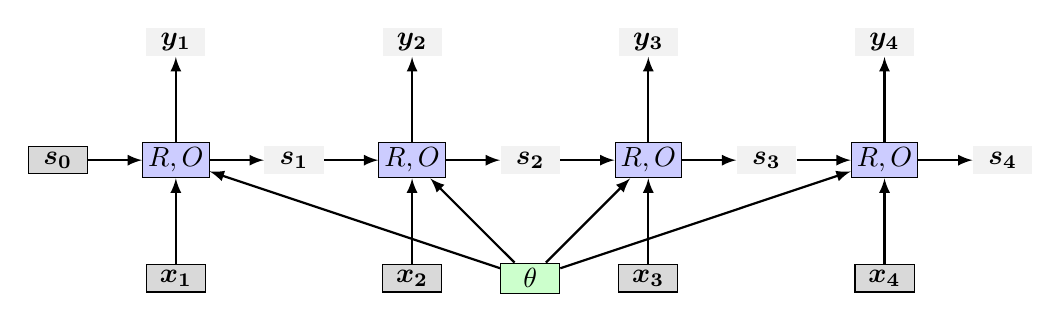
\begin{tikzpicture}	
			%\node (a1) [draw, circle, inner sep=0pt, minimum width=0.75cm, fill=green!20] {$a_1$};
			
			\node (s0) [constant]{$\bm{s_0}$};
			
			\node (ro1) [neuron, right of=s0, xshift=0.5cm] {$R, O$};
			\node (s1) [state, right of=ro1, xshift=0.5cm] {$\bm{s_1}$};
			\node (x1) [constant, below of=ro1, yshift=-0.5cm] {$\bm{x_1}$};
			\node(y1) [state, above of=ro1, yshift=0.5cm] {$\bm{y_1}$};
			
			\node (ro2) [neuron, right of=s1, xshift=0.5cm] {$R, O$};
			\node (s2) [state, right of=ro2, xshift=0.5cm] {$\bm{s_2}$};
			\node (x2) [constant, below of=ro2, yshift=-0.5cm] {$\bm{x_2}$};
			\node(y2) [state, above of=ro2, yshift=0.5cm] {$\bm{y_2}$};
			
			\node (ro3) [neuron, right of=s2, xshift=0.5cm] {$R, O$};
			\node (s3) [state, right of=ro3, xshift=0.5cm] {$\bm{s_3}$};
			\node (x3) [constant, below of=ro3, yshift=-0.5cm] {$\bm{x_3}$};
			\node(y3) [state, above of=ro3, yshift=0.5cm] {$\bm{y_3}$};
			
			\node (ro4) [neuron, right of=s3, xshift=0.5cm] {$R, O$};
			\node (s4) [state, right of=ro4, xshift=0.5cm] {$\bm{s_4}$};
			\node (x4) [constant, below of=ro4, yshift=-0.5cm] {$\bm{x_4}$};
			\node(y4) [state, above of=ro4, yshift=0.5cm] {$\bm{y_4}$};
			
			\node (e) [param, below of=s2, yshift=-0.5cm] {$\theta$};
			
			
			\begin{scope}[thick, black, ->, >=latex]
				\draw (s0) -- (ro1);
				\draw(x1) -- (ro1);
				\draw(e) -- (ro1);
				\draw(ro1) -- (s1);
				\draw(ro1) -- (y1);
				
				\draw (s1) -- (ro2);
				\draw(x2) -- (ro2);
				\draw(e) -- (ro2);
				\draw(ro2) -- (s2);
				\draw(ro2) -- (y2);
				
				\draw (s2) -- (ro3);
				\draw(x3) -- (ro3);
				\draw(e) -- (ro3);
				\draw(ro3) -- (s3);
				\draw(ro3) -- (y3);
				
				\draw (s3) -- (ro4);
				\draw(x4) -- (ro4);
				\draw(e) -- (ro4);
				\draw(ro4) -- (s4);
				\draw(ro4) -- (y4);
				
			\end{scope}
			
		\end{tikzpicture}
		
		Gradients might vanish (become exceedingly close to 0) as they propagate back through the computation graph
		
		\begin{itemize}
			\item Severe in deeper networks, and especially so in recursive and recurrent networks
			\item Hard for the S-RNN to capture long-range dependencies
		\end{itemize}
		
		
		
	\end{frame}
	
	\subsection{Gated architectures}
	
	\begin{frame}{RNN as a general purpose computing device}
		
		State $\bm{s_i}$ represents a finite memory
		
		\begin{block}{Recall: Simple RNN}
			$\bm{s_i} = R(\bm{x_i}, \bm{s_{i - 1}}) = g(\bm{s_{i-1}} \bm{W^s} + \bm{x_i} \bm{W^x} + \bm{b})$ 	
		\end{block}
		\pause
		Each application of function $R$
		\begin{itemize}
			\item Reads the current memory $\bm{s_{i-1}}$
			\item Reads the current input $\bm{x_i}$
			\item Operates on them in some way
			\item Writes the result to the memory $\bm{s_i}$
		\end{itemize}
		\pause Memory access not controlled: At each step, entire memory state is read, and entire memory state is written
	\end{frame}
	
	\begin{frame}{How to provide more controlled memory access?}
		Memory vector $\bm{s} \in \mathbb{R}^d$ and input vector $\bm{x} \in \mathbb{R}^d$
		\pause
		
		Let's have a binary vector (``gate'') $\bm{g} \in \{0, 1\}^d$
		\pause
		\begin{block}{Hadamard-product $\bm{z} = \bm{u} \odot \bm{v}$}
			Fancy name for element-wise multiplication
			$\bm{z_{[i]}} = \bm{u_{[i]}} \cdot \bm{v_{[i]}}$
		\end{block}
		$
		\bm{s'} \gets \bm{g} \odot \bm{x} + (\bm{1} + \bm{g}) \odot \bm{s}
		$
		\begin{itemize}
			\item \pause Reads the entries in $\bm{x}$ corresponding to ones in the gate, writes them to the memory
			\item \pause Remaining locations are copied from the memory
		\end{itemize}
		
	\end{frame}
	
	\begin{frame}{Gate example}
		Updating memory position 2
		$$
		\begin{aligned}
			\begin{pmatrix}
				8 \\ 11 \\ 3
			\end{pmatrix}
			&\gets
			&\begin{pmatrix}
				0 \\ 1 \\ 0
			\end{pmatrix}
			&
			\odot
			&\begin{pmatrix}
				10 \\ 11 \\ 12
			\end{pmatrix}
			&+
			&\begin{pmatrix}
				1 \\ 0 \\ 1
			\end{pmatrix}
			&\odot
			&\begin{pmatrix}
				8 \\ 9 \\ 3
			\end{pmatrix}
			\\
			\bm{s'} &\gets &\bm{g} &\odot &\bm{x} &+ &(\bm{1} + \bm{g}) &\odot &\bm{s} \\
		\end{aligned}
		$$
		\pause
		Could be used for gates in RNNs! But:
		\begin{itemize}
			\item Our gates are not learnable
			\item Our hard-gates are not differentiable
		\end{itemize}
		Solution: Replace with `soft' gates
	\end{frame}
	
	\subsection{LSTM}
	
	\begin{frame}{Long Short-Term Memory (LSTM)}
		Designed to solve the vanishing gradients problem, first to introduce the gating mechanism
		
		\pause
		LSTM splits the state vector $\bm{s_i}$ exactly in two halves
		\begin{itemize}
			\item One half is treated as `memory cells'
			\item The other half is `working memory'
		\end{itemize}
		
		\pause
		\begin{block}{Memory cells}
			\begin{itemize}
				\item Designed to preserve the memory, and also the error gradients, across time
				\item Controlled through \emph{differentiable gating components} --- smooth functions that simulate logical gates
			\end{itemize}
		\end{block}
		
		
	\end{frame}
	
	\begin{frame}{Long Short-Term Memory (LSTM)}
		
		The state at time $j$ is composed of two vectors:
		\begin{itemize}
			\item $\bm{c_j}$ --- the memory component
			\item $\bm{h_j}$ --- the hidden state component
		\end{itemize}
		
		\pause
		At each input state $j$, a gate decides how much of the new input should be written to the memory cell, and how much of the current content of the memory cell should be forgotten
		
		\pause
		There are three gates
		\begin{itemize}
			\item $\bm{i}$ --- input gate
			\item $\bm{f}$ --- forget gate
			\item $\bm{o}$ --- output gate
		\end{itemize}
		
		
	\end{frame}
	
	\begin{frame}{LSTM architecture}
		\begin{figure}
			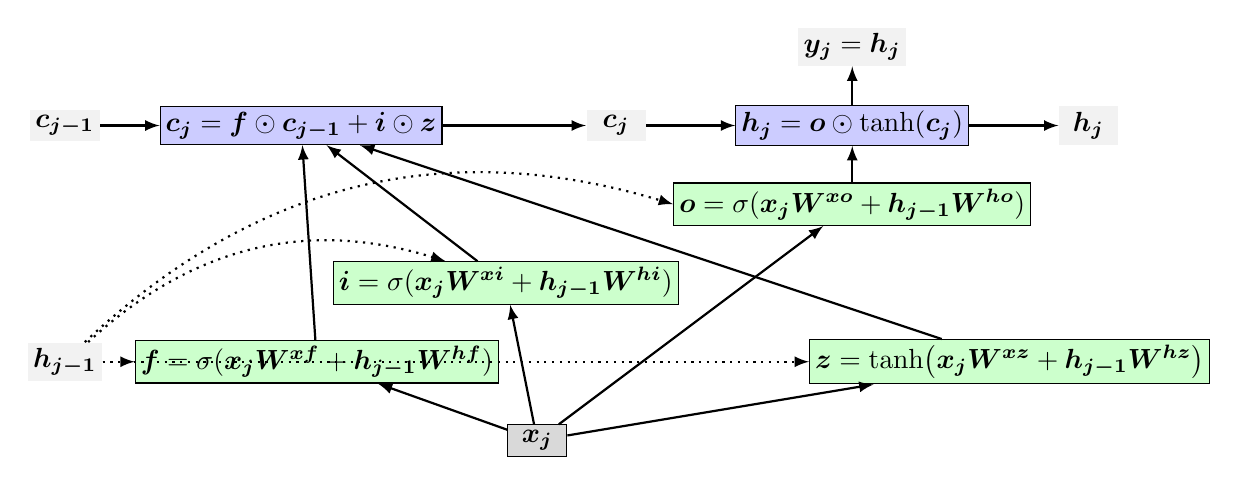
\begin{tikzpicture}	
				
				\onslide<1->{
					\node (c0) [state]{$\bm{c_{j-1}}$};
					\node (h0) [state, below of=c0, yshift=-2cm]{$\bm{h_{j-1}}$};	
					\node (xj) [constant, below of=h0, xshift=6cm] {$\bm{x_j}$};
				}
				
				\onslide<2->{
					\node(z) [param, right of=h0, xshift=11cm] {$\bm{z} = \tanh(\bm{x_j} \bm{W^{xz}} + \bm{h_{j-1} \bm{W^{hz}}} )$};
				}
				
				
				\onslide<3->{
					\node(f) [param, right of=h0, xshift=2.2cm] {$\bm{f} = \sigma(\bm{x_j} \bm{W^{xf}} + \bm{h_{j-1} \bm{W^{hf}}} )$};
				}
				
				\onslide<4->{
					\node(i) [param, right of=h0, xshift=4.6cm, yshift=1cm] {$\bm{i} = \sigma(\bm{x_j} \bm{W^{xi}} + \bm{h_{j-1} \bm{W^{hi}}} )$};
				}
				
				
				\onslide<5->{
					\node(cj) [neuron, right of=c0, xshift=2cm] {$\bm{c_j} = \bm{f} \odot \bm{c_{j-1}} + \bm{i} \odot \bm{z}$};
					
					\node (cjout) [state, right of=cj, xshift=3cm] {$\bm{c_j}$};
				}
				
				\onslide<7->{
					\node(hj) [neuron, right of=cj, xshift=6cm] {$\bm{h_j} = \bm{o} \odot \tanh(\bm{c_j})$};
					
					\node (hjout) [state, right of=hj, xshift=2cm] {$\bm{h_j}$};
				}
				
				\onslide<6->{
					\node(o) [param, below of=hj, xshift=0cm, yshift=0cm] {$\bm{o} = \sigma(\bm{x_j} \bm{W^{xo}} + \bm{h_{j-1} \bm{W^{ho}}} )$};
				}
				\onslide<8->{
					
					\node(yj) [state, above of=hj, yshift=0cm] {$\bm{y_j} = \bm{h_j}$};
				}
				\begin{scope}[thick, black, ->, >=latex]
					
					\onslide<2->{
						\draw(xj) -- (z);
					}
					\onslide<2>{
						\draw [dotted] (h0) -- (z);
					}
					
					\onslide<3->{
						\draw(xj) -- (f);
					}
					\onslide<3>{
						\draw [dotted] (h0) -- (f);
					}
					
					\onslide<4->{
						\draw(xj) -- (i);
					}
					\onslide<4>{
						\draw [dotted] (h0) to [bend left] (i);
					}
					
					\onslide<5->{
						\draw (f) -- (cj);
						\draw (i) -- (cj);
						\draw (z) -- (cj);
						\draw (c0) -- (cj);
						\draw (cj) -- (cjout);
					}
					
					\onslide<6->{
						\draw(xj) -- (o);
					}
					\onslide<6>{
						\draw  [dotted]  (h0) to [bend left] (o.west);
					}
					
					\onslide<7->{
						\draw (o) -- (hj);
						\draw (cjout) -- (hj);
						\draw (hj) -- (hjout);
					}
					
					\onslide<8->{
						\draw (hj) -- (yj);
					}
					
				\end{scope}
				
				
				
			\end{tikzpicture}
		\end{figure}
		
		\onslide<2->{
			$\bm{z}$ --- update candidate
		}
	\end{frame}
	
	\begin{frame}{LSTM parameters and dimensions}
		
		\vspace{-1em}
		$$\bm{x_j} \in \mathbb{R}^{d_{in}} \quad
		\bm{c_j}, \bm{h_j}, \bm{y_j}, \bm{i}, \bm{f}, \bm{o}, \bm{z} \in \mathbb{R}^{d_h} \quad
		\bm{W^{x\star}} \in \mathbb{R}^{d_{in} \times d_{h}} \quad
		\bm{W^{h\star}} \in \mathbb{R}^{d_{h} \times d_{h}}$$
		
		$d_h$ --- dimensionality of LSTM (`hidden' layer)
		
		\vspace{-3em}
		\begin{figure}
			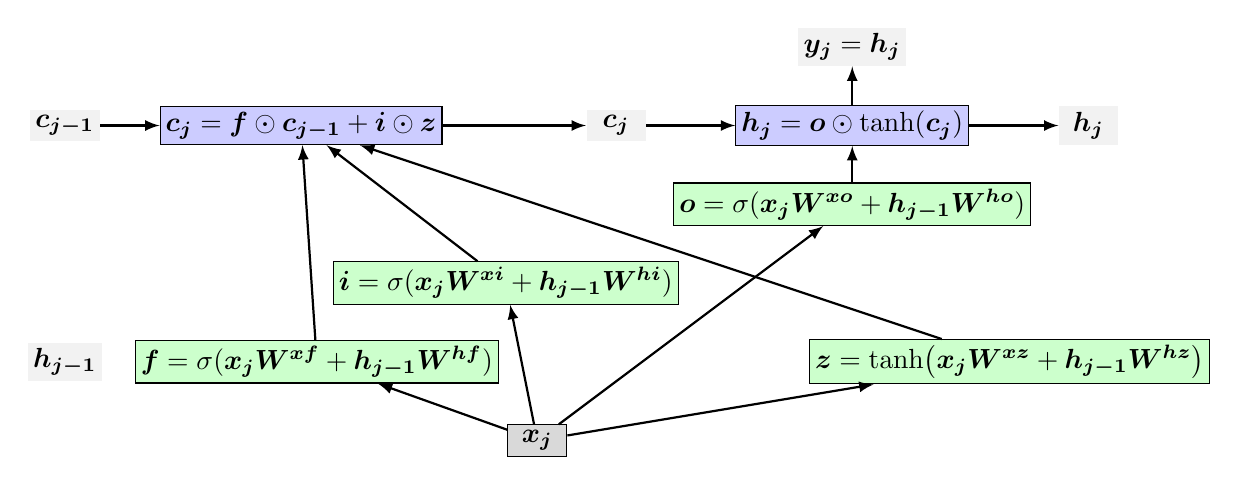
\begin{tikzpicture}	
				
				
				\node (c0) [state]{$\bm{c_{j-1}}$};
				\node (h0) [state, below of=c0, yshift=-2cm]{$\bm{h_{j-1}}$};	
				\node (xj) [constant, below of=h0, xshift=6cm] {$\bm{x_j}$};
				\node(z) [param, right of=h0, xshift=11cm] {$\bm{z} = \tanh(\bm{x_j} \bm{W^{xz}} + \bm{h_{j-1} \bm{W^{hz}}} )$};
				\node(f) [param, right of=h0, xshift=2.2cm] {$\bm{f} = \sigma(\bm{x_j} \bm{W^{xf}} + \bm{h_{j-1} \bm{W^{hf}}} )$};
				\node(i) [param, right of=h0, xshift=4.6cm, yshift=1cm] {$\bm{i} = \sigma(\bm{x_j} \bm{W^{xi}} + \bm{h_{j-1} \bm{W^{hi}}} )$};
				\node(cj) [neuron, right of=c0, xshift=2cm] {$\bm{c_j} = \bm{f} \odot \bm{c_{j-1}} + \bm{i} \odot \bm{z}$};
				
				\node (cjout) [state, right of=cj, xshift=3cm] {$\bm{c_j}$};
				\node(hj) [neuron, right of=cj, xshift=6cm] {$\bm{h_j} = \bm{o} \odot \tanh(\bm{c_j})$};
				
				\node (hjout) [state, right of=hj, xshift=2cm] {$\bm{h_j}$};
				\node(o) [param, below of=hj, xshift=0cm, yshift=0cm] {$\bm{o} = \sigma(\bm{x_j} \bm{W^{xo}} + \bm{h_{j-1} \bm{W^{ho}}} )$};
				
				\node(yj) [state, above of=hj, yshift=0cm] {$\bm{y_j} = \bm{h_j}$};
				
				\begin{scope}[thick, black, ->, >=latex]
					
					
					\draw(xj) -- (z);
					\draw(xj) -- (f);
					\draw(xj) -- (i);
					\draw (f) -- (cj);
					\draw (i) -- (cj);
					\draw (z) -- (cj);
					\draw (c0) -- (cj);
					\draw (cj) -- (cjout);
					\draw(xj) -- (o);
					\draw (o) -- (hj);
					\draw (cjout) -- (hj);
					\draw (hj) -- (hjout);
					\draw (hj) -- (yj);
					
					
				\end{scope}
				
				
				
			\end{tikzpicture}
		\end{figure}
		
		
	\end{frame}
	
	
	\begin{frame}{LSTM as a `layer'}
		
		\begin{figure}
			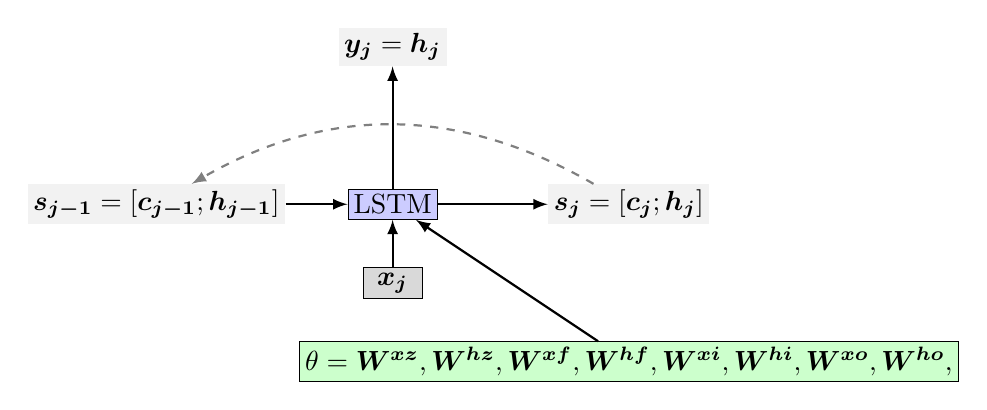
\begin{tikzpicture}	
				%\node (a1) [draw, circle, inner sep=0pt, minimum width=0.75cm, fill=green!20] {$a_1$};
				
				\node (s0) [state]{$\bm{s_{j-1}} = [\bm{c_{j-1}}; \bm{h_{j-1}} ]$};
				
				\node (ro) [neuron, right of=s0, xshift=2cm] {LSTM};
				\node (si) [state, right of=ro, xshift=2cm]{$\bm{s_{j}} = [\bm{c_{j}}; \bm{h_{j}} ]$};
				\node (xi) [constant, below of=ro] {$\bm{x_{j}}$};
				\node(yi) [state, above of=ro, yshift=1cm] {$\bm{y_j} = \bm{h_j}$};
				
				\node (e) [param, below of=si, yshift=-1cm] {$\theta = \bm{W^{xz}}, 
					\bm{W^{hz}},
					\bm{W^{xf}},
					\bm{W^{hf}},
					\bm{W^{xi}},
					\bm{W^{hi}},
					\bm{W^{xo}},
					\bm{W^{ho}},
					$};
				
				
				\begin{scope}[thick, black, ->, >=latex]
					\draw (s0) -- (ro);
					\draw(xi) -- (ro);
					\draw(e) -- (ro);
					\draw(ro) -- (si);
					\draw(ro) -- (yi);
				\end{scope}
				\draw [thick, dashed, gray, ->, >=latex] (si) to [bend right] (s0);
				
			\end{tikzpicture}
		\end{figure}
		
		We also ignored bias terms for each gate
	\end{frame}
	
	
	\section*{Recap}
	
	% **Content**
	%
	%* Vanilla RNNs (and maybe vanishing/exploding gradient?)
	%* LSTM cells
	%* Bi-Directional LSTMs
	%* Domain adaptation and multi-task learning (?) 
	%
	%**Notes**
	%
	%efficiency, bidirectionality, multi-layer RNNs, how to apply to different tasks, how to ensure no data leakage
	%connection to LMs (using RNNs)?
	%
	%* Domain adaptation and multi-task learning (?) - should be somewhere early too
	
	\begin{frame}{Take aways}
		
		\begin{itemize}
			\item RNNs for arbitrary long input
			\item Encoding the entire sequence and/or each step
			\item Modeling freedom with bi-directional RNNs
			\item Vanishing gradients in deep nets --- gating mechanism, memory cells
			\item LSTM a particularly powerful RNN
		\end{itemize}
		
	\end{frame}
	
	
	
	\begin{frame}{License and credits}
		
		\begin{columns}
			\begin{column}{0.7\textwidth}
				Licensed under Creative Commons Attribution-ShareAlike 4.0 International (CC BY-SA 4.0)
			\end{column}
			\begin{column}{0.2\textwidth}
				
\includegraphics[width=0.9\linewidth]{img/cc-by-sa-icon.pdf}
			\end{column}
		\end{columns}
		
		\bigskip
		
		Credits
		
		\begin{scriptsize}
			
			Ivan Habernal
			
			Content from ACL Anthology papers licensed under CC-BY \url{https://www.aclweb.org/anthology}
			
			
		\end{scriptsize}
		
	\end{frame}
	
	
	
\end{document}

